\documentclass{article}
% \author{Risto Virtaharju and Olli Mustajoki}
% Set page size and margins
% Replace `letterpaper' with `a4paper' for UK/EU standard size
\usepackage[a4paper,top=2cm,bottom=2cm,left=2cm,right=2cm,marginparwidth=1.75cm]{geometry}


% Emerald Harvard Citation Style

\usepackage[style=authoryear,backend=biber,natbib=true,maxcitenames=2,uniquelist=false,style=ieee]{biblatex}
\addbibresource{ML2024.bib} % your .bib file

\usepackage[parfill]{parskip} % New line, no indent for paragraph breaks
\usepackage{pdfpages}
\usepackage{amstext}
\usepackage{graphicx}

\begin{document}
%Front Matter

\title{A Machine Learning Approach to Classifying Billiards Balls}
\maketitle

\section{Introduction}
This report is about recognizing billiard balls from images. Our student organization has an interest for software that can analyze billiard games from video footage. Currently, our billiard statistics software only registers the outcomes, without insights into the gameplay itself. A system capable of recognizing the balls on the table could generate various player statistics, such as the success rate of long shots or games lost due to potting the eight ball prematurely. As a first step towards developing this system, this project focuses specifically on labeling individual billiards balls from clear, square-shaped images.

This report is structured as follows: First, the problem is defined, including an overview of the dataset and the machine learning approach. The methodology section details the data preprocessing, model selection, and the training process. This is followed by a discussion of the results, including evaluation metrics and insights gained from the experiments. Finally, conclusions and potential areas for improvement are outlined.



\section{Problem Formulation}
\label{sec:problem_formulation}
Our dataset of billiards balls contains 960 high-quality 3552x3552 pixel, 24-bit RGB images of billiards balls, 60 for each of the 16 different categories. Each image only depicts one ball. The data is therefore categorical with 16 different classes, one representing each type of ball.

We have cropped and resized the images to 64 by 64 pixels. We have also scaled the color 8-bit color channels, whose values range from 0 to 256, to floating-point values between 0 and 1. After preprocessing the image dataset, each image will constitute a $3\times 4096$ feature matrix of floating-point values. A machine learning model, specifically a SVM classifier, is trained using this labeled dataset. This means we have a supervised machine learning task, with the goal of accurately predicting the labels of input images. 

\section{Method}
\label{sec:method}
A large literature of image classification projects exist. In this report we implement two approaches for image classification: a support vector machine classifier (SVC) and a convolutional neural network (CNN). For the SVC approach we have chosen to largely follow the method described in \cite{unknownMachineLearningApproach2023}. The CNN approach largely follows tensorflow's computer vision tutorial, which we also used for the dataset loading and preprocessing \cite{ComputerVisionTensorFlow}.

\subsection{Dataset}
\label{sec:dataset}
The dataset of billiards ball images was created specifically for the goal of predicting the correct labels of billiards balls at our table location. We took 60 photos of each of the 16 balls from various angles, resulting in 960 total images. The images taken were 3552 by 3552 pixel jpg images with a bit depth of 24. The dataset was split into training, validation and test datasets. The final training dataset had 720 images, validation dataset 80 images and test dataset 160 images, corresponding roughly to a 75-8-17 split. We chose this split to have most of the data be used in training, while setting aside separate datasets for validation to prevent overfitting, and testing to evaluate the final performance of the model. The reasoning for a commonly used 75-10-15 split is explained in \cite{josephOptimalRatioData2022}. The training, validation and test datasets were randomly separated using scikit-learn's train\_test\_split-function.

\subsection{Data Preprocessing and Feature Engineering}
\label{sec:data_preprocessing}
\subsubsection*{Preprocessing}
\label{sec:preprocessing}
Our initial dataset consists of unnecessarily large RGB images. Our preprocessing has three steps: Cropping the images, resizing them to 64x64 pixels and scaling the 8-bit integer RGB values down to a single floating-point number between 0 and 1. This is done to reduce the size of inputs to the model from an integer matrix of size $3\times(3552^2)$, to a more manageable $3\times 4096$ floating-point values. The color value scaling was done because machine learning methods generally work better with small input values. \cite{ImportanceFeatureScaling}. Now each feature is a 3 by 4096 matrix of floating-point numbers between 0 and 1. The dimensions of the matrix represent the red, green and blue color channels of the image. The features are labeled with a number between 0 and 15, representing the ground truth, which is the number of the billiards ball in the image. The cue ball is number 0.

\subsubsection*{Principal Component Analysis}
\label{sec:principal_component_analysis}
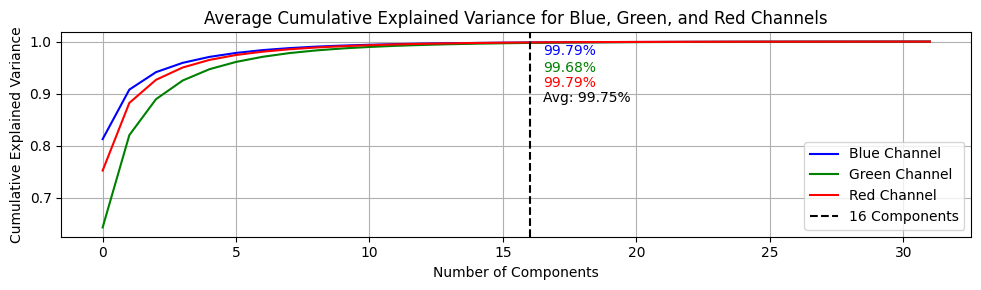
\includegraphics[width=\textwidth]{images/pca_cumulative_variance.png}
With the Support Vector Classifier (explained in section \ref{sec:svm_classifier}), the data was additionally preprocessed with Principal Component Analysis (PCA) in order to reduce input feature size \cite{woldPrincipalComponentAnalysis}. We chose the number of PCA components to be 16, based on our analysis of cumulative explained variance of the number of components for each color channel over the training dataset. 16 PCA components explained 99,75\% of variance in the images. This reduced the size of the features by 75\% from $64\times64\times3$ to $64\times16\times3$. The PCA was implemented using the PCA class of scikit-learn’s decomposition module \cite{PCA}.

\subsubsection*{Data Augmentation}
\label{sec:data_augmentation}
We used data augmentation when training our CNN model (explained in section \ref{sec:convolutional_neural_network}). We chose to perform the augmentation since our dataset is comparatively small and not very diverse. We augmented the training dataset by applying random rotations, image flips and brightness adjustments to the preprocessed training dataset images. The augmentation was performed using keras' layers utility \cite{ModuleTfkeraslayersTensorFlow}. We also found that augmentation greatly reduced model overfitting to the training dataset.

\subsection{Model}
\label{sec:model}
\subsubsection*{SVM Classifier}
\label{sec:svm_classifier}
For this task of recognizing billiard balls from images, we have selected the Support Vector Classifier (SVC) as our initial ML model. SVC is ideal for handling high-dimensional data, like images, by finding a hyperplane that maximises the margin between different classes. In this case, the classes are different billiard balls. SVC works by identifying the optimal weight vector and bias term to separate these classes. If the data isn't linearly separable, kernel functions such as the Radial Basis Function (RBF) can be used to map the data to a higher-dimensional space, allowing more accurate classification. \cite{unknownMachineLearningApproach2023, nobleWhatSupportVector2006}

\begin{equation}
    h(x)=sign(wx+b)
\end{equation}

In this case, $h(x)$ assigns a class label  to the input data point $x$, returning +1 when $wx+b$ is greater than or equal to 0, and -1 when it is less than 0.

SVC was chosen because of its ability to efficiently manage image-based tasks with numerous pixel features, and its effectiveness in separating classes through margin maximization. It's also robust against overfitting and performs well with smaller datasets like the couple thousand images used in this project, making it a practical and reliable choice. \cite{unknownMachineLearningApproach2023,nobleWhatSupportVector2006}

\subsubsection*{Convolutional Neural Network}
\label{sec:convolutional_neural_network}
For this project, we also implemented a Convolutional Neural Network (CNN), another powerful machine learning model designed specifically for image-based tasks. CNNs are highly effective in recognizing patterns within images by taking advantage of their unique architecture, which is well-suited for extracting spatial hierarchies from visual data \cite{osheaIntroductionConvolutionalNeural2015}.

A CNN works by passing the input image through several layers, including convolutional layers, pooling layers, and fully connected layers. The convolutional layers apply filters that move across the image to detect local features such as edges or textures. These features are then aggregated in the pooling layers, which reduce the spatial dimensions of the data, preserving important information while minimizing computational complexity. The final fully connected layers perform the actual classification by combining the learned features into predictions for each class \cite{osheaIntroductionConvolutionalNeural2015}.

We tested three different CNN models. The first model had three convolutional layers with 16, 32, and 64 filters (3x3 kernels, ReLU activation), each followed by max pooling. The output was flattened and passed through a 128-unit dense layer with ReLU activation, and then a final dense layer with 16 outputs for classification. The second model, model\_l2, was identical to the first but applied L2 kernel regularization to the 128-unit dense layer. The third model, model\_batch, introduced batch normalization between each layer. We used regularization and normalization to reduce overfitting. As outlined in the results, the three models performed very similarly, all achieving over 95\% test accuracy.

\subsection{Loss Function}
\label{sec:loss_function}
\subsubsection*{SVM Hinge Loss}
\label{sec:svm_hinge_loss}
For this project, we have selected the hinge loss function as our initial loss function, which is commonly used with Support Vector Machines (SVMs). Hinge loss encourages the model to maximize the margin between different classes, penalizing predictions that fall too close to the decision boundary or are misclassified. This ensures that the SVC model not only classifies the billiard balls correctly but does so with confidence, reducing the likelihood of errors. \cite{unknownMachineLearningApproach2023, bartlettClassificationRejectOption2008}

\begin{equation}
    L(y, f(x)) = max(0, 1-y \cdot f(x))
\end{equation}

Here, $y$ denotes the actual class label (+1 or -1), while $f(x)$ refers to the classifier's decision function for the given data point $x$.

Hinge loss is computationally efficient and aligns perfectly with SVC's margin-maximizing objective, making it an ideal choice. By penalizing near-boundary predictions, hinge loss ensures that the model maintains clear and accurate boundaries between billiard ball classes, improving overall classification performance. \cite{unknownMachineLearningApproach2023, bartlettClassificationRejectOption2008}

\subsubsection*{CNN Sparse Multiclass Cross Entropy}
\label{sec:cnn_sparse_multiclass_cross_entropy}
For our Convolutional Neural Network (CNN), we used the Sparse Multiclass Cross-Entropy Loss function to optimize the model’s performance in the classification of billiard balls. This loss function is specifically designed for multiclass classification tasks where each image corresponds to exactly one class, making it well-suited for our project of recognizing a single billiard ball from each image \cite{jeevaLossFunctionsNeural2023}.

The Sparse Multiclass Cross-Entropy Loss works by comparing the true class label with the predicted probability for that class. The function takes the negative log of the predicted probability assigned to the true class, and then averages this value across the dataset. Mathematically, it is expressed as:
\begin{equation}
    L(y_{\text{true}}, y_{\text{pred}}) = - \sum (y_{\text{true}} \times \log(y_{\text{pred}}))
\end{equation}

Here, $y_{\text{true}}$ represents the true label (an integer value between 0 and the number of classes), while $y_{\text{pred}}$ is the predicted probability for that class. This formulation ensures that the model is penalized more when it assigns a lower probability to the correct class\cite{jeevaLossFunctionsNeural2023}.

One advantage of the sparse version of cross-entropy loss is its computational efficiency, as it only requires the probability for the true class rather than for all possible classes. However, it is somewhat less robust to class imbalance than other loss functions, which could be considered in future iterations of the project. Overall, Sparse Multiclass Cross-Entropy Loss allowed us to efficiently train the CNN while maintaining a high level of prediction accuracy.

\section{Results}
\label{sec:results}
The results of this project demonstrate the performance of both the Support Vector Classifier (SVC) and Convolutional Neural Network (CNN) in recognizing billiard balls from images. We present the evaluation metrics, including accuracy, training time, and prediction time, for each model configuration.

\subsection*{Support Vector Classifier}

The SVC was evaluated with and without Principal Component Analysis (PCA) to assess the trade-offs between accuracy and computational efficiency. As we can see from the results below, the training time increased by a factor of 26 and prediction time by a factor of 52. While accuracy improves without PCA, the computational cost in terms of time is drastically higher. The decision to use PCA thus depends on the project's priorities, whether focusing on accuracy or efficiency.

\begin{table}[h]
    \centering
    \begin{tabular}{|c|c|c|c|}
        \hline
        Dataset & With PCA (16 components) & Without PCA & Change \\ 
        \hline
        Train & 91.53\% & 89.03\% & -2.5\% \\ 
        Validation & 80.00\% & 85.00\% & +5\% \\ 
        Test & 70.00\% & 81.25\% & +11.25\% \\ 
        \hline
        Training time$^{*}$ & 11 seconds & 4 minutes 47 seconds & $\times 26$ \\
        Prediction time$^{*}$ & 3 seconds & 2 minutes 36 seconds & $\times 52$ \\
        \hline
    \end{tabular}
    \caption{SVC prediction accuracy and computation times with and without PCA.}
    \label{table:accuracy_pca}
\end{table}

$^{*}$ Prediction time reported her means the time to predict labels for the testing dataset of 160 images. The training time with PCA includes the time for performing PCA on the training dataset. The reason for the difference in relative computation times with and without PCA between training and prediction is because the prediction time doesn't include the time used to perform PCA on the test dataset.

\subsection*{Convolutional Neural Network}

\begin{figure}[h]
    \centering
    \begin{minipage}{0.32\textwidth}
        \centering
        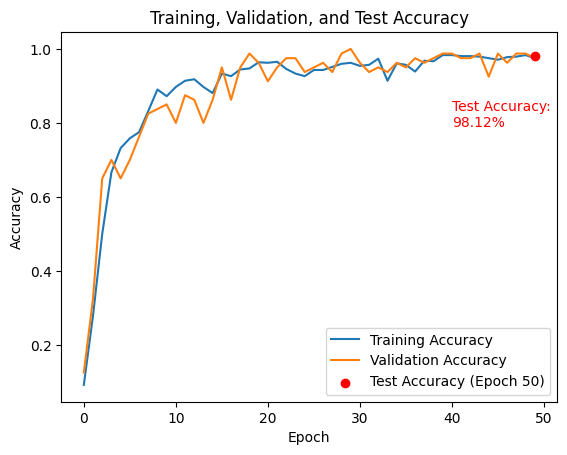
\includegraphics[width=\textwidth]{images/cnn_accuracy.png}
    \end{minipage}
    \hfill
    \begin{minipage}{0.32\textwidth}
        \centering
        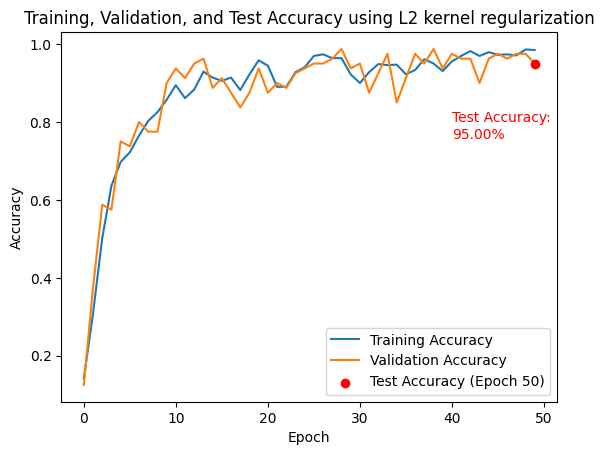
\includegraphics[width=\textwidth]{images/l2_cnn_accuracy.png}
    \end{minipage}
    \hfill
    \begin{minipage}{0.32\textwidth}
        \centering
        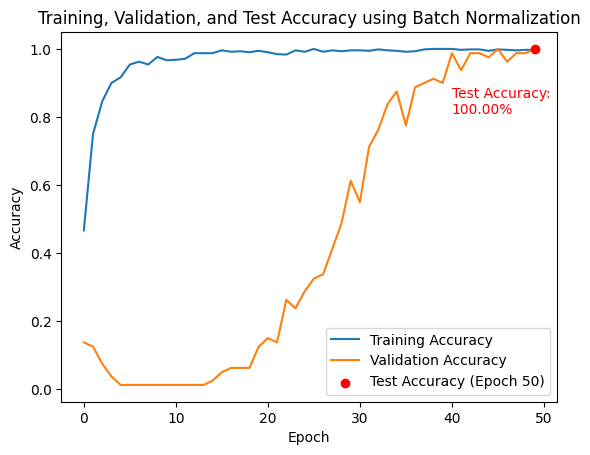
\includegraphics[width=\textwidth]{images/batch_cnn_accuracy.png}
    \end{minipage}
\end{figure}

The graph above shows the performance of the three CNN models over their training period of 50 epochs each. Model\_batch performed the best, but all models achieved over 95\% accuracy. When running the training multiple times, the results weren't stable, but landed somewhere above 95\%. Further statistical analysis of the difference in model performance could be done, but we have chosen to not include that in this project. We cannot currently say that there is any significant difference between the three CNN models tested.

\section{Conclusion}
\label{sec:conclusion}
In this report, we explored two machine learning models—Support Vector Classifier (SVC) and Convolutional Neural Network (CNN)—to classify billiard balls from images. The SVC provided a computationally efficient method for classification, although its accuracy was lower compared to the CNN models. The CNN models, in contrast, achieved higher classification accuracy, surpassing 95\% on the test dataset.

Despite the promising results, there are areas for improvement. The relatively small size and lack of diversity in the dataset limited the models’ generalizability. Future work could explore expanding the dataset with additional variations, such as different lighting conditions and more complex backgrounds. The scope of the machine learning problem could also be widened to include image segmentation and object detection to find coordinates of multiple billiards balls from an image.

Overall, this project successfully demonstrated the potential of machine learning for automating the recognition of billiard balls. The work presented here can serve as a first step toward more advanced applications.

\pagebreak
\section{Aknowledgements}
\textbf{\textit{Use of generative AI}}

Parts of this text were generated using ChatGPT, but all prompts were crafted and texts edited and reviewed the authors. Additionally, ChatGPT was used for assistance in data processing and coding.


\printbibliography


\appendix
\section{preprocessing.pdf}

% 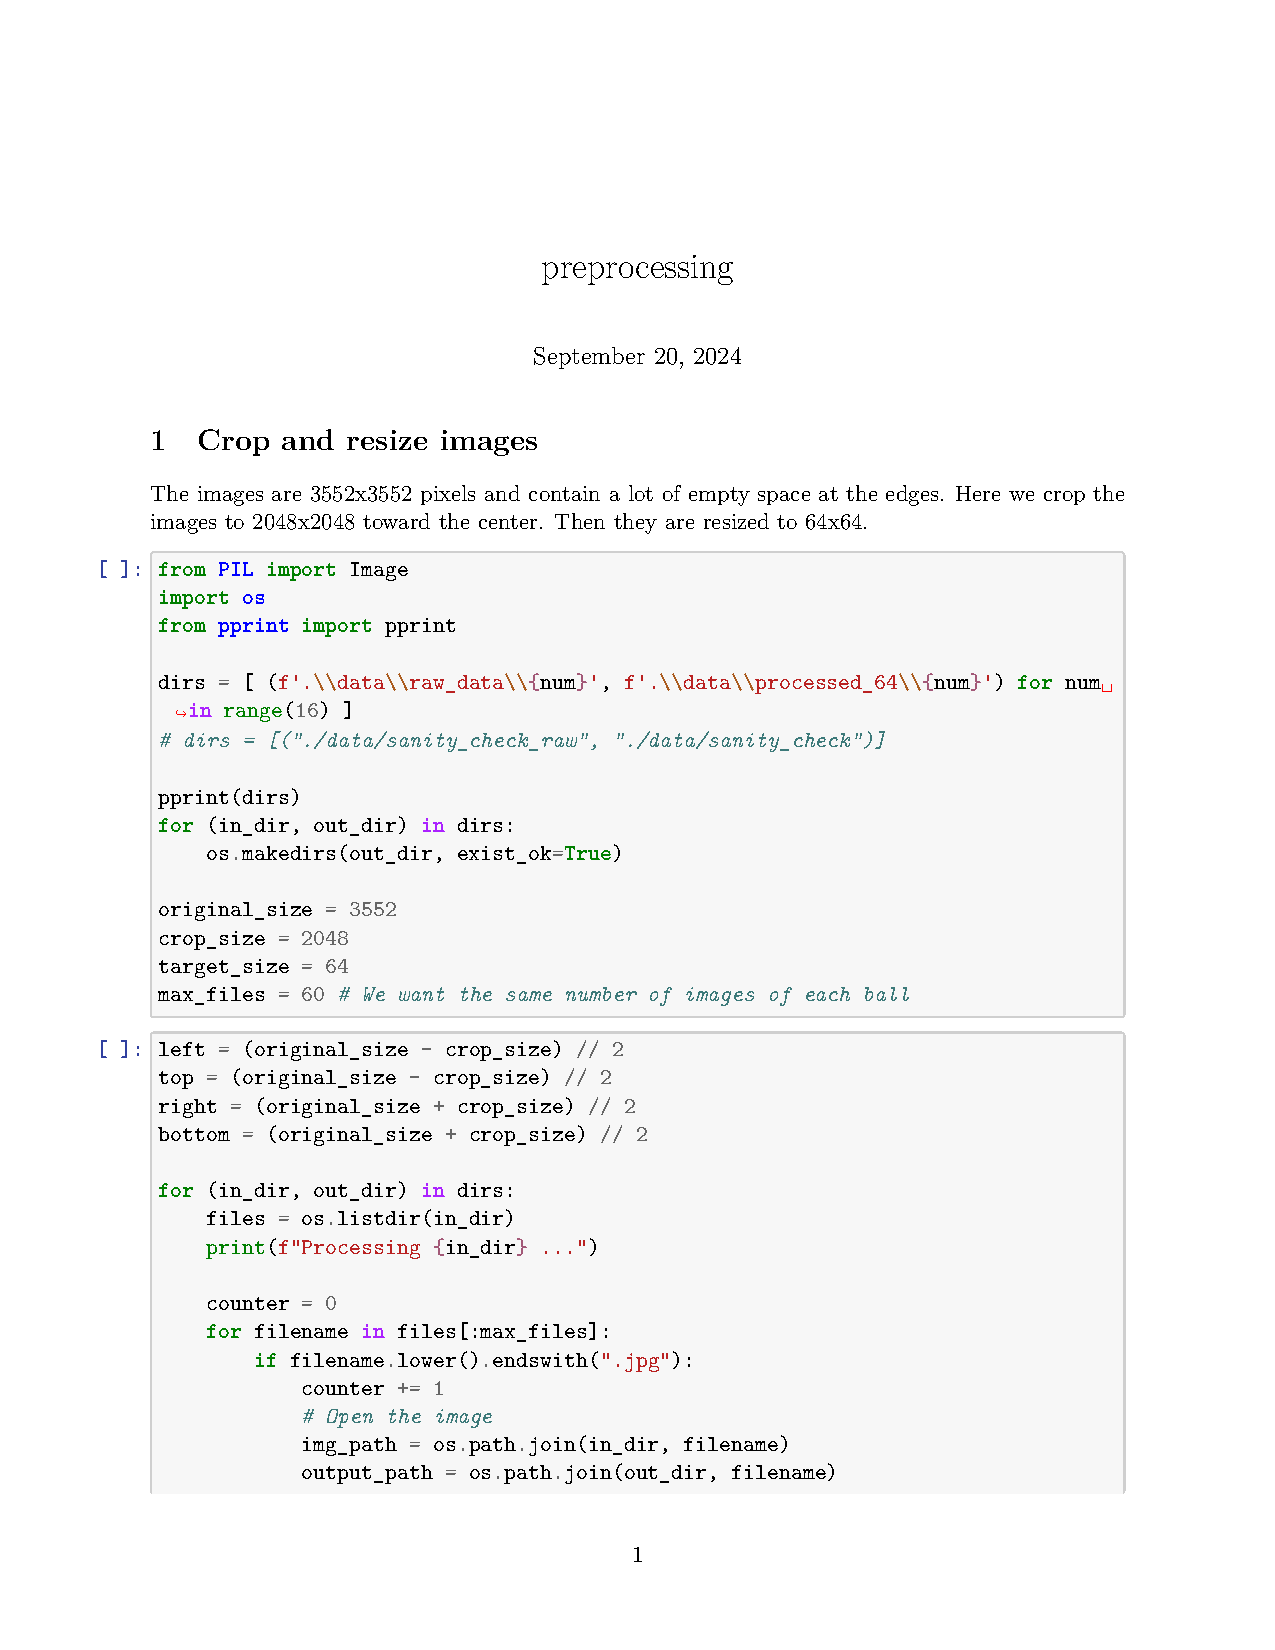
\includepdf[pages=-]{preprocessing.pdf}

\end{document}
